% Created 2025-03-14 Fri 12:20
% Intended LaTeX compiler: pdflatex
\documentclass[smaller]{beamer}\usepackage{listings}
\usepackage{color}
\usepackage{amsmath}
\usepackage{array}
\usepackage[T1]{fontenc}
\usepackage{natbib}
\lstset{
keywordstyle=\color{blue},
commentstyle=\color{red},stringstyle=\color[rgb]{0,.5,0},
literate={~}{$\sim$}{1},
basicstyle=\ttfamily\small,
columns=fullflexible,
breaklines=true,
breakatwhitespace=false,
numbers=left,
numberstyle=\ttfamily\tiny\color{gray},
stepnumber=1,
numbersep=10pt,
backgroundcolor=\color{white},
tabsize=4,
keepspaces=true,
showspaces=false,
showstringspaces=false,
xleftmargin=.23in,
frame=single,
basewidth={0.5em,0.4em},
}
\usepackage{natbib, dsfont, pgfpages, tikz,amssymb, amsmath,xcolor}
\bibliographystyle{abbrvnat}
\usetikzlibrary{shapes.geometric, arrows}
\tikzstyle{startstop} = [rectangle, minimum width=1cm, minimum height=1cm,text centered, align=center]
\tikzstyle{process} = [rectangle, minimum width=3cm, minimum height=1cm, text centered, draw=black]
\tikzstyle{arrow} = [thick,->,>=stealth]
\usepackage{prodint}
\setbeamertemplate{footline}[frame number]
\beamertemplatenavigationsymbolsempty
\usepackage{appendixnumberbeamer}
\setbeamercolor{gray}{bg=white!95!black}
\setbeamertemplate{itemize items}{$\circ$}
\lstset{basicstyle=\ttfamily\footnotesize}
\RequirePackage{fancyvrb}
\DefineVerbatimEnvironment{verbatim}{Verbatim}{fontsize=\footnotesize}
\renewcommand*{\thefootnote}{\fnsymbol{footnote}}
\setbeamerfont{footnote}{size=\scriptsize}
\definecolor{bblue}{rgb}{0.2,0.2,0.7}
\newcommand{\E}{{\ensuremath{\mathop{{\mathbb{E}}}}}}
\newcommand{\R}{\mathbb{R}}
\newcommand{\N}{\mathbb{N}}
\newcommand{\blank}{\makebox[1ex]{\textbf{$\cdot$}}}
\newcommand\independent{\protect\mathpalette{\protect\independenT}{\perp}}
\def\independenT#1#2{\mathrel{\rlap{$#1#2$}\mkern2mu{#1#2}}}
\renewcommand{\phi}{\varphi}
\renewcommand{\epsilon}{\varepsilon}
\newcommand*\diff{\mathop{}\!\mathrm{d}}
\newcommand{\weakly}{\rightsquigarrow}
\newcommand\smallO{\textit{o}}
\newcommand\bigO{\textit{O}}
\newcommand{\midd}{\; \middle|\;}
\newcommand{\1}{\mathds{1}}
\usepackage{ifthen} %% Empirical process with default argument
\newcommand{\G}[2][n]{{\ensuremath{\mathbb{G}_{#1}}{\left[#2\right]}}}
\DeclareMathOperator*{\argmin}{\arg\!\min}
\DeclareMathOperator*{\argmax}{\arg\!\max}
\newcommand{\V}{\mathrm{Var}} % variance
\newcommand{\eqd}{\stackrel{d}{=}} % equality in distribution
\newcommand{\arrow}[1]{\xrightarrow{\; {#1} \;}}
\newcommand{\arrowP}{\xrightarrow{\; P \;}} % convergence in probability
\newcommand{\KL}{\ensuremath{D_{\mathrm{KL}}}}
\newcommand{\leb}{\lambda} % the Lebesgue measure
\DeclareMathOperator{\TT}{\Psi} % target parameter
\newcommand{\empmeas}{\ensuremath{\mathbb{P}_n}} % empirical measure

\renewcommand*\familydefault{\sfdefault}
\itemsep2pt
\usepackage[utf8]{inputenc}
\usepackage[T1]{fontenc}
\usepackage{graphicx}
\usepackage{longtable}
\usepackage{wrapfig}
\usepackage{rotating}
\usepackage[normalem]{ulem}
\usepackage{amsmath}
\usepackage{amssymb}
\usepackage{capt-of}
\usepackage{hyperref}
\usetheme{default}
\author{Anders Munch \newline \small joint work with Thomas Gerds \newline \newline Section of Biostatistics, UCPH}
\date{March 20, 2025}
\title{Targeted learning with right-censored data using the state learner}
\begin{document}

\maketitle

\begin{frame}[label={sec:org3c06c93}]{Targeted or debiased machine learning}
Low-dimensional target parameter
\begin{equation*}
  \Psi \colon \mathcal{P}
  \rightarrow \R,
  \quad \text{such that} \quad
  \Psi(P) =
  \tilde{\Psi}(\nu_1(P), \dots , \nu_B(P)),
\end{equation*}
for high-dimensional nuisance parameters \(\nu_1, \dots,
\nu_B\).

\vfill

(Picture from PhD with multi-state model)
\end{frame}

\begin{frame}[label={sec:orgea38621}]{Examples of estimands}
Available data \(O = (X, \tilde{T}, \tilde{D}) \sim P \in
\mathcal{P}\), where
\begin{align*}
  X & = W \in \R^d \text{ or } X=(W,A) \in \R^d\times \{0,1\},
  \\
  \tilde{T} & = T \wedge C
  \\
  \tilde{D} & = \1{\{T \leq C\}}D, \quad D = 1 \text{ or } D \in \{1,2\}.
\end{align*}

The variables \(T\) and \(D\) are the uncensored event time and
event indicator.

\vfill

\begin{overlayarea}{\textwidth}{0.4\textheight}
  \only<2>{
    \begin{beamercolorbox}[rounded=true]{gray}
      \begin{equation*}
        Q(T > t)
        % =
        % \E_Q{[Q(T > t \mid X)]}
        \stackrel{(!)}{=}
        \E_P{[e^{-\Lambda_P(t \mid X)}]},
        \quad (T,X) \sim Q,
      \end{equation*}
      where
      \begin{equation*}
        \Lambda_P(\diff t \mid x) = P(\tilde{T} \in \diff t,
        \tilde{D}  = 1
        \mid \tilde{T} \geq t, X=x).
      \end{equation*}
      For (!) to hold we need \( C \independent T \mid X \).
    \end{beamercolorbox}
  }

  \only<3>{
    \begin{beamercolorbox}[rounded=true]{gray}
      Use \( \{(T^a, D^a) : a \in \{0,1\}\} \sim Q\), to
      denote potential outcomes.
      \begin{equation*}
        Q(T^{a} \leq t, D^{a} = 1)
        \stackrel{(!)}{=}
        % \int_{\mathcal{W}}
        % \int_0^t e^{-[\Lambda_{1,P}+\Lambda_{2,P}](u \mid
        %   a, w)} \Lambda_{1,P}(\diff u \mid a, w)
        % P_W(\diff w)
        \E_{P}{
          \left[
            \int_0^t e^{-[\Lambda_{1,P}+\Lambda_{2,P}](u \mid
              a, W)} \Lambda_{1,P}(\diff u \mid a, W)
          \right]},
      \end{equation*}
      % where
      \begin{equation*}
        \Lambda_{d,P}(\diff t \mid a, w) = P(\tilde{T} \in \diff t,
        \tilde{D}  = d
        \mid \tilde{T} \geq t, A=a, W=w).
      \end{equation*}
      For (!) to hold we need both
      \( C \independent T \mid X \) and causal assumptions.
    \end{beamercolorbox}
  }
\end{overlayarea}
\end{frame}

\begin{frame}[label={sec:org2118e05}]{Targeted learning with super learning}
\begin{equation*}
  \Psi(P) = \E_{P}{
    \left[
      \int_0^t e^{-[\Lambda_{1,P}+\Lambda_{2,P}](u \mid
        a, W)} \Lambda_{1,P}(\diff u \mid a, W)
    \right]}  
\end{equation*}
can be written as
\begin{equation*}
  \Psi(P) = \tilde{\Psi}(\Lambda_{1,P}, \Lambda_{2,P}, P_W).
\end{equation*}

\vfill

\begin{beamercolorbox}[rounded=true]{gray}
\begin{center}
  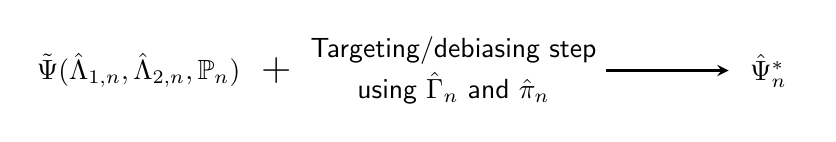
\begin{tikzpicture}
    \node (A) [startstop]
    {$\tilde{\Psi}(\hat{\Lambda}_{1,n}, \hat{\Lambda}_{2,n},
      \empmeas)$}; \node (B) [startstop, right of=A,
    xshift=3cm] {Targeting/debiasing step \\[0.1cm]
      using $\hat{\Gamma}_n$ and  $\hat{\pi}_n$}; \node
    (C) [startstop, right of=B, xshift=3cm]
    % {\( \hat{\Psi}_n^{\text{TMLE}} \),
    % \( \hat{\Psi}_n^{\text{DML}} \)};
    { \( \hat{\Psi}_n^* \)};

    \node (plus) [right of=A, xshift=.75cm] {\Large +};

    % Arrows
    \draw [arrow] (B.east) -- (C.west);
  \end{tikzpicture}
\end{center}
\end{beamercolorbox}

\begin{block}{}
Asymptotic valid inference and \(\bigO_P(n^{-1/2})\) convergence
for \(\hat{\Psi}_n^*\) if
\begin{equation*}
  \| \hat{\nu}_n - \nu \|_{P,2} = \smallO_P{(n^{-1/4})},
  \quad \text{for all } \hat{\nu}_n \in
  \{ \hat{\Lambda}_{1,n}, \hat{\Lambda}_{2,n}, \hat{\Gamma}_n,
  \hat{\pi}_n \}.
\end{equation*}

\vfill

To achieve this we can use a super learner to data-adaptively
select an estimator from a library of candidates.
\end{block}
\end{frame}

\begin{frame}[label={sec:org3012b9a}]{Super learning\footnote{\cite{stone1974cross,geisser1975predictive,wolpert1992stacked,breiman1996stacked,van2007super}}}
\begin{onlyenv}<1>

\begin{center}
  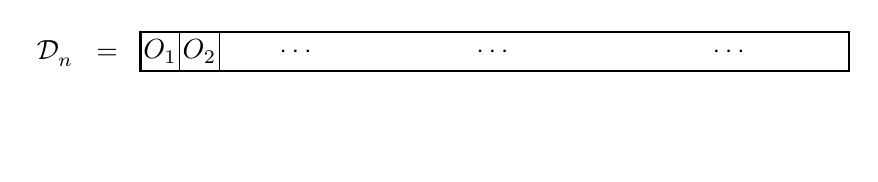
\begin{tikzpicture}
      \node at (-.8,0.25) {\( \mathcal{D}_n^{\phantom{-1}} = \)};
      \node at (-.8,-0.75) {\phantom{\( \mathcal{D}_n^{1} = \)}};
      % Draw consecutive boxes without spaces
      \draw[thick,color=white] (0,-1) rectangle ++(3,.5);
      \draw[thick] (0,0) rectangle ++(9,.5);
      % \draw[thick] (3,0) rectangle ++(3,.5);
      % \draw[thick] (6,0) rectangle ++(3,.5);
      \draw (0,0) rectangle ++(0.5,0.5);
      \draw (.5,0) rectangle ++(0.5,0.5);
      \node at (0.25,0.25) {$O_1$};
      \node at (0.75,0.25) {$O_2$};
          
      \node at (2,0.25) {\dots};
      \node at (4.5,0.25) {\dots};
      \node at (7.5,0.25) {\dots};

    \end{tikzpicture}
\end{center}
\end{onlyenv}


\begin{onlyenv}<2>

\begin{center}
  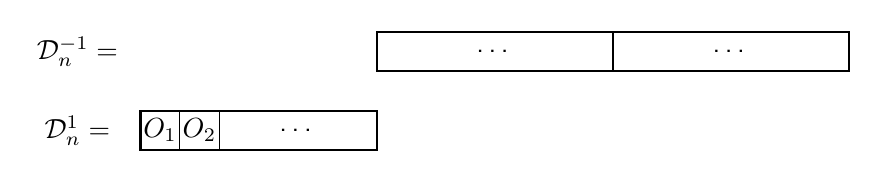
\begin{tikzpicture}
      \node at (-.8,0.25) {\( \mathcal{D}_n^{-1} = \)};
      \node at (-.8,-0.75) {\( \mathcal{D}_n^{1} = \)};
      % Draw consecutive boxes without spaces
      \draw[thick] (0,-1) rectangle ++(3,.5);
      \draw[thick] (3,0) rectangle ++(3,.5);
      \draw[thick] (6,0) rectangle ++(3,.5);
      \draw (0,-1) rectangle ++(0.5,0.5);
      \draw (.5,-1) rectangle ++(0.5,0.5);
      \node at (0.25,-0.75) {$O_1$};
      \node at (0.75,-0.75) {$O_2$};
          
      \node at (2,-0.75) {\dots};
      \node at (4.5,0.25) {\dots};
      \node at (7.5,0.25) {\dots};

    \end{tikzpicture}
\end{center}
\end{onlyenv}


\begin{onlyenv}<3->

\begin{center}
    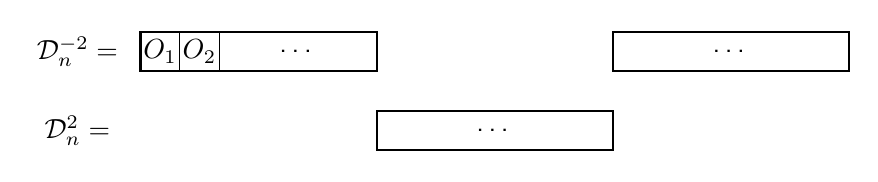
\begin{tikzpicture}
      % Draw consecutive boxes without spaces
      \node at (-.8,0.25) {\( \mathcal{D}_n^{-2} = \)};
      \node at (-.8,-0.75) {\( \mathcal{D}_n^{2} = \)};
      
      \draw[thick] (0,0) rectangle ++(3,.5);
      \draw[thick] (3,-1) rectangle ++(3,.5);
      \draw[thick] (6,0) rectangle ++(3,.5);
      \draw (0,0) rectangle ++(0.5,0.5);
      \draw (.5,0) rectangle ++(0.5,0.5);
      \node at (0.25,0.25) {$O_1$};
      \node at (0.75,0.25) {$O_2$};
          
      \node at (2,0.25) {\dots};
      \node at (4.5,-0.75) {\dots};
      \node at (7.5,0.25) {\dots};

    \end{tikzpicture}
\end{center}
\end{onlyenv}

\begin{block}{\color{white}{dummy}}
\begin{description}
\item[{Learner}] \(\mathcal{D}_n \longmapsto a(\mathcal{D}_n) = \hat
  \nu_n\)
\item[{Library}] \(\mathcal{A} = \{a_1, a_2, \dots, a_M \}\)
\item[{Loss function}] \(\mathcal{V} \times \mathcal{O} \ni (\nu,
  O) \longmapsto L(\nu, O) \in \R\)
\end{description}

\begin{equation*}
  \text{Discrete SL} = \hat{a}_n = \argmin_{a \in \mathcal{A}}
  \frac{1}{K}\sum_{k=1}^{K}
  \frac{1}{| \mathcal{D}_n^{k} |}\sum_{O_i \in \mathcal{D}_n^{k}}
  L
  {
    \left(
      a{ (\mathcal{D}_n^{-k})}
      , O_i
    \right)
  },
\end{equation*}
\end{block}
\end{frame}

\begin{frame}[label={sec:org29d1562}]{\color{white} breaker}
\begin{beamercolorbox}[rounded=true]{gray}
\centering \Large Evaluating performance in hold-out folds is
a challenge with right-censored data
\end{beamercolorbox}
\end{frame}

\begin{frame}[label={sec:org8427469}]{The negative log-likelihood is unsuited for super learning}
\begin{center}
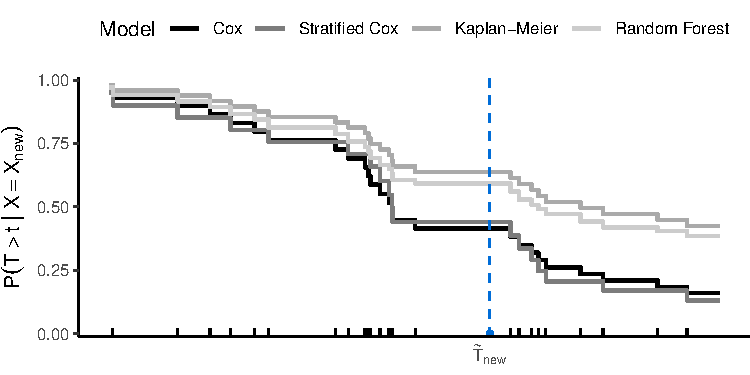
\includegraphics[width=0.9\textwidth]{./sl-hold-out-sample.pdf}
\end{center}
\end{frame}

\begin{frame}[label={sec:org18db45c}]{\large IPCW and pseudo-outcome require pre-specified censoring estimator}
\def\shift{3}
\def\ls{}
\def\lw{.5mm}
\centering \Large
  \begin{tikzpicture}
    \node[] (S) at (0,\shift) {$\widehat S$};
    \node[] (WG) at (\shift,\shift) {$\widehat{W}_{G}$};
    \node[] (G) at (\shift,0) {$\widehat G$};
    \node[] (WS) at (0,0) {$\widehat{W}_{S}$};
    \draw[<-, \ls, line width=\lw, gray] (S) to[out=30,in=150] (WG);
    \draw[<-, \ls, line width=\lw, gray] (WG) to[out=30-90,in=150-90] (G);
    \draw[<-, \ls, line width=\lw, gray] (G) to[out=30-180,in=150-180] (WS);
    \draw[<-, \ls, line width=\lw, gray] (WS) to[out=30-270,in=150-270] (S);
  \end{tikzpicture}
\end{frame}


\begin{frame}[label={sec:org2d13ae0}]{The state learner: Model all `states' of the \emph{observed} data}
\begin{equation*}
  N(t) = \1{
    \{
      \tilde{T} \leq t, \tilde D=1
    \}} + 2\,\1{\{\tilde{T} \leq t, \tilde
    D=2\}} - \1{\{\tilde{T} \leq t, \tilde D=0\}}
  % \in \{-1, 0, 1, 2\}
\end{equation*}

\vfil

\begin{center}
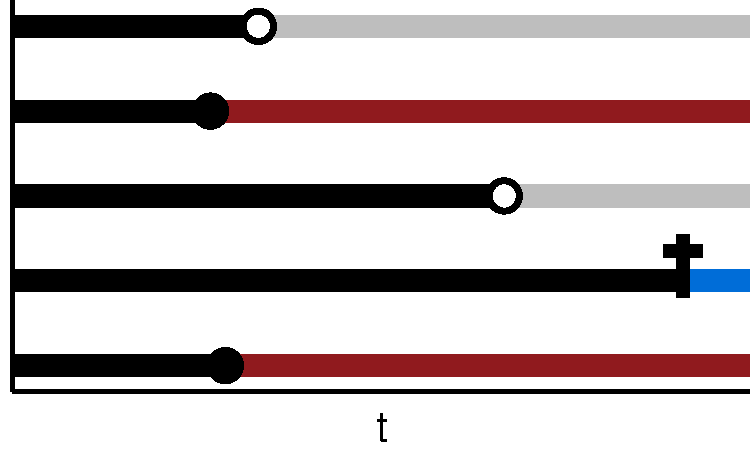
\includegraphics[width=0.5\textwidth]{./multi-state-data-3-up.pdf}
\end{center}

\vfil

Build a super learner for the function
\begin{equation*}
    F(t, k, w,a) = P(N(t) = k \mid W=w, A=a).
\end{equation*}
\end{frame}

\begin{frame}[label={sec:org68e1cbf}]{Back and forth calculations}
Use
\begin{align*}
  F(t, 0, w,a)
  &
  % =P{\left( \tilde{T}>t \midd W=w,A=a \right)}
    = \Prodi_0^t
    \left( 1 - 
    \left[\Lambda_{1} + \Lambda_{2} + \Gamma
    \right](\diff s \mid w,a) \right),
  \\
  F(t, j, w,a)
  &
  % = P{\left(
    % \tilde{T} \leq t, \Delta=j \midd W=w, A=a
    % \right)}
    = \int_0^t F(t-,0, w,a)  \Lambda_{j}(\diff s \mid w,a),
    \quad  j \in \{1,2\},
  \\
  F(t, -1, w,a)
  &
  % =
    % P{\left( \tilde{T} \leq t, \Delta=0 \midd W=w, A=a \right)}
    = \int_0^tF(t-,0, w,a)  \Gamma(\diff s \mid w,a),
\end{align*}
to build a library for \(F\) from libraries for \(\Lambda_1\), \(\Lambda_2\), \(\Gamma\),
\begin{equation*}
  \mathcal{F}(\mathcal{A}, \mathcal{B}, \mathcal{C})
  = \{ F_{a, b, c} : a \in \mathcal{A}, b \in \mathcal{B},
  c \in \mathcal{C}\}.
\end{equation*}

\pause

\begin{beamercolorbox}[rounded=true]{gray}
\begin{equation*}
  L(F,O) =  \int_0^{\tau} \sum_{j=-1}^{2}
  \Bigl(
    F(t,j,W,A) - \1{\{N(t)=j\}}
    \Bigr)^2
    \diff t.
\end{equation*}
\end{beamercolorbox}
\end{frame}

\begin{frame}[label={sec:org419040c}]{Illustration with data from a prostate cancer study\footnote{\cite{kattan2000pretreatment}.}}
\begin{onlyenv}<1>
\begin{center}
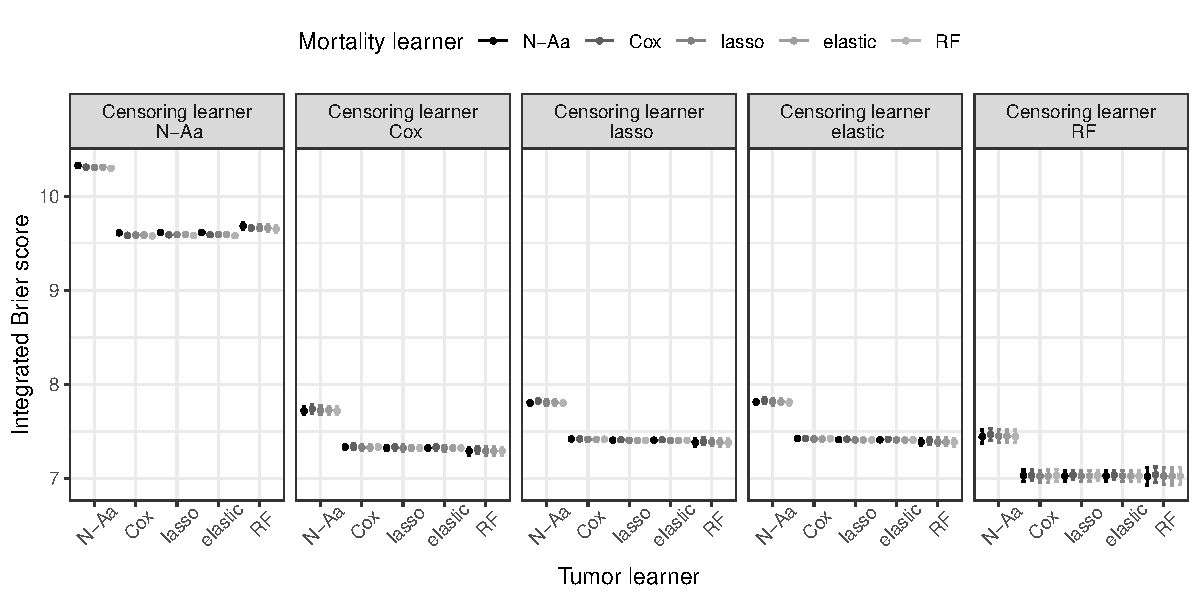
\includegraphics[width=1\textwidth]{./real-data-state-learner.pdf}
\end{center}
\end{onlyenv}

\begin{onlyenv}<2>
\begin{center}
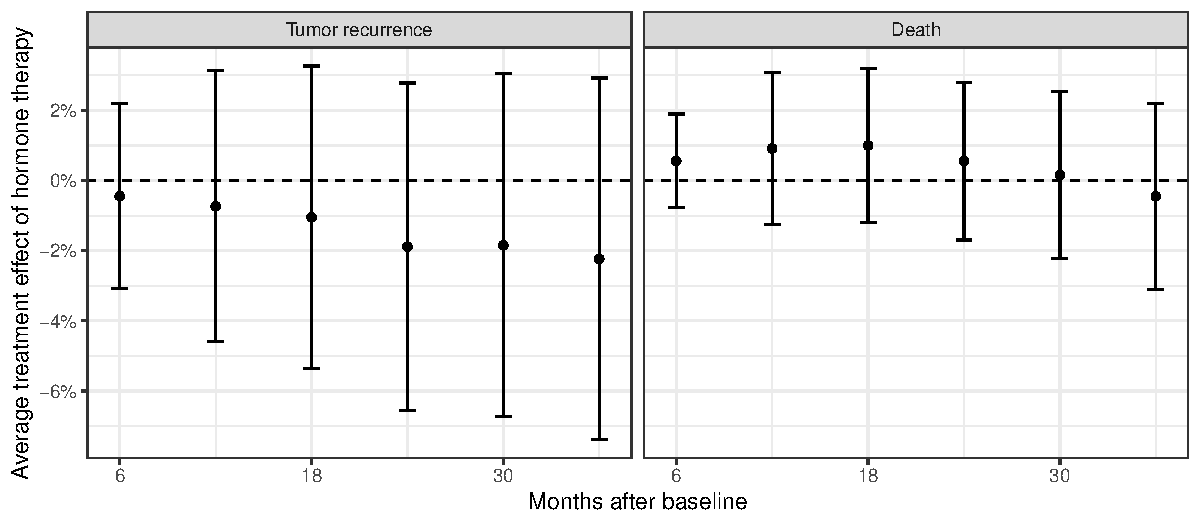
\includegraphics[width=1\textwidth]{./real-data-target.pdf}
\end{center}
\end{onlyenv}
\end{frame}

\begin{frame}[label={sec:orgbcd1621}]{Theoretical results etc -- reference to paper Github}
\end{frame}

\begin{frame}[label={sec:orgc4aaa09}]{References}
\footnotesize \bibliography{bib.bib}
\end{frame}
\end{document}